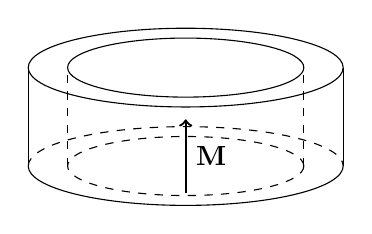
\begin{tikzpicture}
\def\leng {4}
\def\hgt {1.25}
\def\xrad {0.5}
\def\yrad {0.125}
\def\innerRatio {0.75}

% Draw ring
\draw (0,0.5*\hgt) circle [x radius = \xrad*\leng, y radius = \yrad*\leng];
\draw (-0.5*\leng,-0.5*\hgt) -- (-0.5*\leng,0.5*\hgt);
\draw (0.5*\leng,-0.5*\hgt) -- (0.5*\leng,0.5*\hgt);
\draw (-0.5*\leng,-0.5*\hgt) arc[x radius = \xrad*\leng, y radius = \yrad*\leng, start angle = -180, end angle = 0];
\draw[dashed] (-0.5*\leng,-0.5*\hgt) arc[x radius = \xrad*\leng, y radius = \yrad*\leng, start angle = 180, end angle = 0];
\draw[dashed] (0,-0.5*\hgt) circle [x radius = \innerRatio*\xrad*\leng, y radius = \innerRatio*\yrad*\leng];
\draw (0,0.5*\hgt) circle [x radius = \innerRatio*\xrad*\leng, y radius = \innerRatio*\yrad*\leng];
\draw[dashed] (-\innerRatio*\xrad*\leng,-0.5*\hgt) -- (-\innerRatio*\xrad*\leng,0.5*\hgt);
\draw[dashed] (\innerRatio*\xrad*\leng,-0.5*\hgt) -- (\innerRatio*\xrad*\leng,0.5*\hgt);

% Magnetisation vector
\draw[->,thick] (0,-0.5*\innerRatio*\hgt-\yrad*\leng) -- (0,0.5*\innerRatio*\hgt-\yrad*\leng) node[right,pos=0.5] {\(\mathbf{M}\)};

\end{tikzpicture}